\section{Ocean Models}
\lastupdated{2024-11-30 18.45 }{CMN}


Similar equation to the atmosphere but with significant differences that lead to different scales for time and space
but as for the atmosphere, the scales of primary importance are those that respond to low frequencies and larger scale motions; the time scales in the oceans are much longer than those in the atmosphere because of the greater thermal inertia, the horizontal length scales are 1/10 of the atmosphere. One measure of the relevant horizontal length scales is the radius of deformation L defined as the ratio of the phase speed of gravity waves c(gr) to the corioli's parameter:  \(L=Cgr/f\)
The radiative flux is less complex.
Water motion is constrained by bottom topography.
the hydrostatic approximation is even better.
sea water is nearly incompressible, so the equation of continuity can be abbreviated by eliminating the time change of density, although density variations are generally included as far as buoyancy effects are concerned. By eliminating the derivative of density, it becomes:

\begin{figure}[htp!]
	\centering
	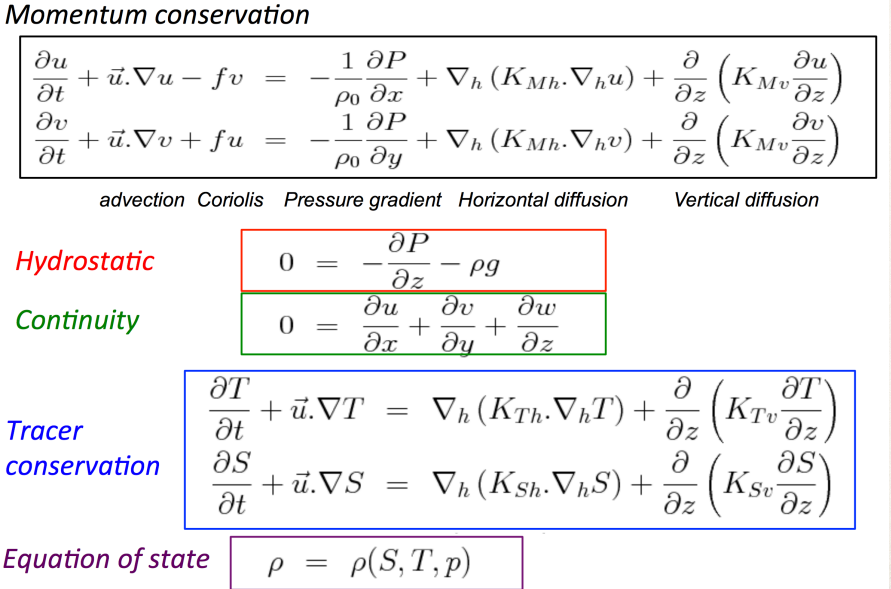
\includegraphics[width=0.5\linewidth]{uploads/Screenshot 2024-11-21 225126.png}
	\caption{Equations in ocean dynamics}
	\label{fig:equations in ocean dyn}
\end{figure}
\begin{figure}[htp!]
	\centering
	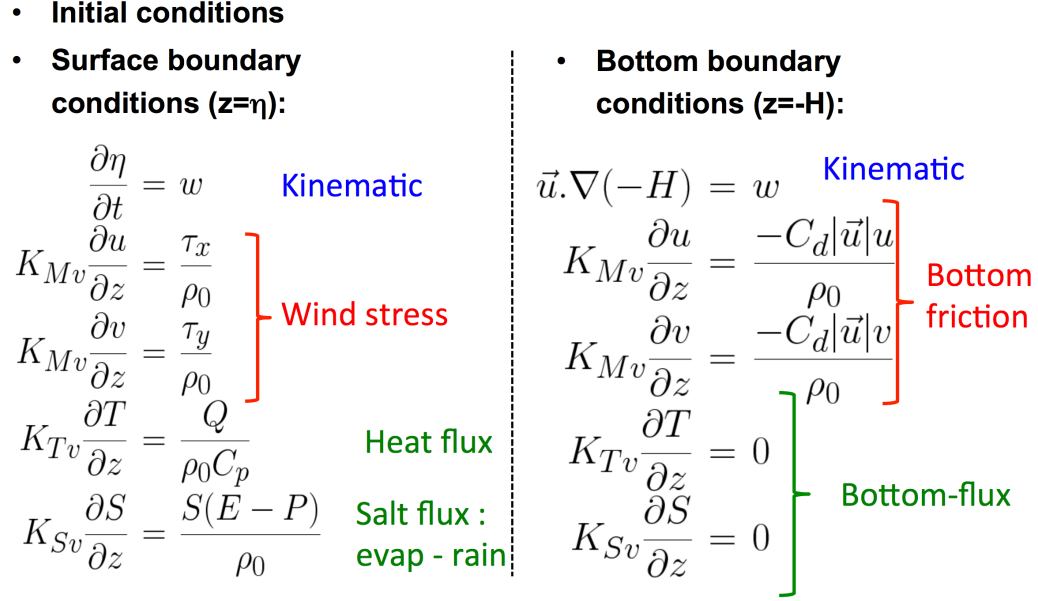
\includegraphics[width=0.5\linewidth]{uploads/Screenshot 2024-11-21 225410.png}
	\caption{Boundary conditions}
	\label{fig:boundary conditions}
\end{figure}
ice models are somewhat different from ocean models because it is not a fluid anymore but a solid, discontinuous in nature , varying in its distribution from one time period to another. in contrast to ocean and atmospheric models, whose calculations center on determine the properties of the water--air, sea ice have the primary goal of determine the location and each time step.  including ice thickness and aerial ice concentration. Calculation for climate oriented sea ice models can be divided into two categories, (1) calculations concerned with the thermodynamics of ice cover, the thickness and temperature structure of the ice, based on the principle of the conservation of energy(2) calculations concerned with ice dynamic.  determing the motion of the ice based on the conservation of momentum.
(for more details on thermodynamics\&dynamics pag 129-146 book)
River transport system
is an importart
Two possible grids: structured grids (cartesian, curvilinear) for global ocean, basin scale, coastal applications e.g. NEMO, MOM, ROMS, ecc; and unstructured grids, which domain is titled using more general geometrical shapes (triangles, ...) pieced together to optimally fit details of the geometry $\rightarrow$ tidal modelling, near shores, estuaries e.g. FVCOM, FESOM, MPAS, ecc.
\subsubsection{Regular grids}
\begin{itemize}
	\item regular spaced lines;
	\item on a spherical earth cannot have both uniform grid spacing and straight lines $\rightarrow$ grids tend to be curvilinear and the grid cell area tends to vary;
	\item lat-lon regular grids also have a problem at the poles where grid lines converge
	\item they are computationally efficient;
	\item have a relatively straightforward analysis algorithm;
	\item have benefited from decades of research experience
\end{itemize}
but for a given latitude they have a fixed resolution: to increase resolution near the edge of an ocean basin (where you want it!) requires an increase of resolution everywhere including out in the middle of the ocean (where you don't!). An example are the tripolar grids: regular grid laid over the high latitude North Hemisphere region with two rotated poles located over land.
\subsection{Unstructured grids}
\begin{itemize}
	\item irregular grids are designed to give more freedom to put spatial resolution where you want it
	\item a common scheme is composed as a series of triangles = finite elements
	\item by varying the size we can construct a non-uniform horizontal resolution over the computational domain
	\item they are efficient owing to the fact that resolution can be tailored to need as a function of space
	\item they can accurately represent highly irregular coastlines and topography (no need fro "staircase" coasts and topography)
\end{itemize}
but they have unresolved issues with flows dominated by geostrophy and advection (characteristics of large-scale ocean flows), and they have spacially variable resolution-dependent physics (e.g. viscosity and diffusivity coefficients should really be resolution dependent).
\paragraph{Adaptive Grids.} Unstructured meshes with a dynamically changing resolution responding to the nature of flow in time, they are very cool but very much in its infancy for ocean modeling approximations.
\begin{figure}[htp!]
	\centering
	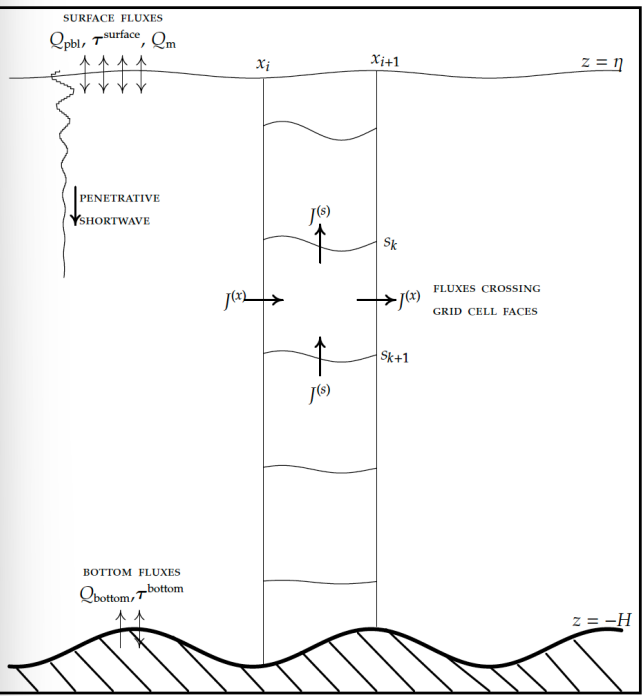
\includegraphics[width=0.40\linewidth]{uploads/Screenshot 2024-11-21 235405.png}
	\caption{Vertical Grids}
	\label{fig:vertical grids}
\end{figure}
\subsubsection{Vertical Grids} The choice of the vertical coordinate system is loaded because the oceans are forced at the surface (most of the action occurs there), they are strongly stratified and they are adiabatic in the interior. There is complex bottom bathymetry to deal with. As a consequence there exist a number of approaches to choose from.

A different choice for the vertical coordinates can be done:
\begin{itemize}
	\item Geopotential or Pressure: common for non-hydrostatic process modelling and large-scale climate modelling (\textcolor{Blue}{MITgcm},\textcolor{Blue}{MOM}, \textcolor{Blue}{NEMO})
	\item Isopycnal:  clean representation of interior quasi-adiabatic flows and overflows (\textcolor{Blue}{GOLD}, \textcolor{Blue}{HYCOM})
	\item Sigma: common for shelf/coastal modelling (\textcolor{Blue}{ROMS})
\end{itemize}
\paragraph{Geopotential Coordinates.} Absolute depth/z-coordinate system. These are based on a serie of depth levels, it is common to add vertical resolution near the surface by decreasing the spacing between the levels in the upper ocean relative to the deep. Most common method for global models.
\begin{itemize}
	\item \textsc{advantages}: simple to set up, computationally efficient, there are no pressure gradient errors.
	\item \textsc{disadvantages}: increased vertical resolution near the lateral boundaries (i.e. continental slopes) requires the addition of grid cells throughout the basin; spurious diapycnal mixing associated with the numerical advection scheme.
\end{itemize}
\paragraph{Sigma.} Terrain following or $\sigma$-coordinate system. It is based on the frational depth, scaled from 0 to 1: $0.01\sigma$ level is $1\%$ of the depth of the ocean, while $0.99\sigma$ level is at 99\% of the depth of the ocean. Applications for shelves and coastal areas.
\begin{itemize}
	\item \textsc{advantages}: mimics the bathymetry and allows high resolution near the sea floor regardless of depth or proximity to land.
	\item \textsc{disadvantages}: pressure gradient errors, issues with spurious diapycnal mixing coming from the numerical advection scheme
\end{itemize}
\paragraph{Isopycnal vertical coordinates.} Density ($\rho$)/"layered models". The vertical grid is defined by density surfaces, it exploits the fact that below the mixed layer, ocean currents generally flow along surfaces of equal density (flow is "adiabatic").
\begin{itemize}
	\item \textsc{advantages}: simple, "exactly isopycnal"
	\item \textsc{disadvantages}: perform poorly where the ocean is less stratified (e.g. in shallow water); no resolution in an unstratified fluid; no mixed layer unless you tack one on; issues with entrainment.
\end{itemize}
\begin{figure}[htp!]
	\centering
	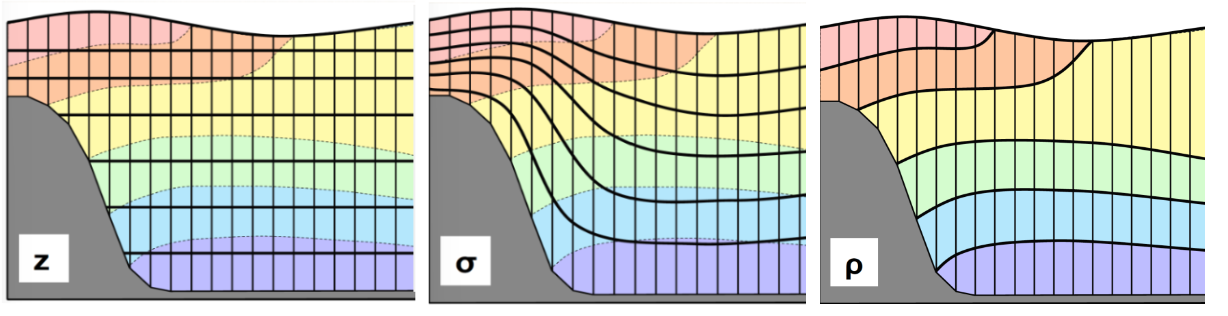
\includegraphics[width=0.5\linewidth]{uploads/Screenshot 2024-11-22 001323.png}
	\caption{$z$, $\sigma$ and isopycnal coordinate systems}
	\label{fig:enter-label}
\end{figure}
\paragraph{Hybrid coordinates.} It seeks to optimize performance by combining the best suited system in different regions based on the dominant processes at work. HYCOM=z coordinates in the surface mixed layer and density coordinates in the stratified ocean below. Here the vertical coordinates evolve in both time and space as the depth of the mixed layer changes.
\begin{itemize}
	\item \textsc{advantages}: dynamically optimized coordinate system gives improved results.
	\item\textsc{disadvantages}: high computational costs.
\end{itemize}

\begin{figure}[htp!]
	\centering
	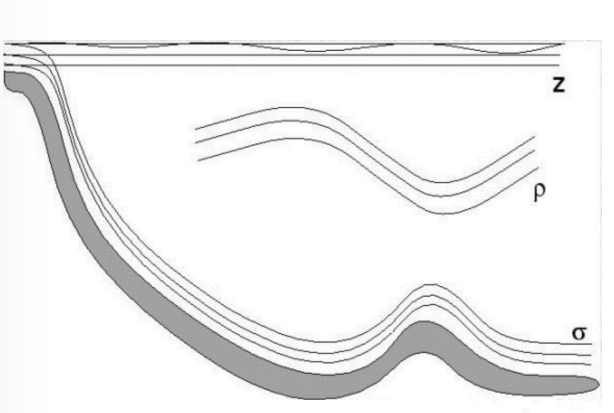
\includegraphics[width=0.5\linewidth]{uploads/Screenshot 2024-11-22 000943.png}
	\caption{Hybrid coordinates}
	\label{fig:enter-label}
\end{figure}
\subsection{Resolution and mesoscale eddies}
\begin{centering}
	"Eddy-resolving" at 1/10° is not enough to resolve ocean "weather"
\end{centering}
\\[0.25 cm]

\textcolor{Blue}{Eddies} are swirling, circular movements of water in the ocean, resembling whirlpools, but they can vary greatly in size and duration. They are a fundamental aspect of ocean dynamics, transporting heat, nutrients, salt, and momentum across the ocean. Eddies often form due to shear instabilities (differences in velocity between layers), boundary currents (for instance Gulf Stream) and topography
The horizontal resolution needed to resolve the first barolinic deformation radius with two grid points.
\begin{itemize}
	\item[$\blacksquare$] there are different rules of thumb: one is that it takes 5 grid points to accurately define a feature without aliasing: this means 1/8° global resolution (\~15 km) can accurately depict only features larger than \~60 km
	\item[$\blacksquare$] models with variable grid spacing have variable resolution - beware of resolution dependent physics!
	\item[$\blacksquare$] resolution is not cheap - because of the CFL (NB. no transport faster than one grid cell per time step) condition, as we shrink the horizontal grid spacing we must add vertical layers and decrease the time step
\end{itemize}
At all (present-day) resolution, OGCMs resolve the mesoscale in some regions but not others.
Global ocean models often describe their horizontal
resolution with respect to their ability to permit or
resolve mesoscale (i.e. Rossby radius scale) eddies. Eddy-resolving does NOT mean all eddies are resolved or that all eddy effects of resolved eddies are acting. The spatial resolution of the ocean component of CMIP5/CMIP6 coupled models is 0.2° to 2°/0.1° to 1°: from coarse (no eddies) to eddy-permitting (partially resolved eddy field). The effects of eddies need to be parameterized in coarse models (more later!); what to do in models that partially resolve the eddy field is an increasingly important question.
\subsubsection{Parametrizations}
Processes need to be parametrized in a model for two reasons:
\begin{enumerate}
	\item we don't spend the computational resources required to directly treat them because they are either too small or too complex.
	\item we don't understand it well enough to be represented by an equation
\end{enumerate}
Processes commonly parametrized in ocean models include: mesoscale eddy effects - submesoscale eddy effects - dense
overflows - coastal processes - surface mixed layer processes
- friction - sub-grid scale mixing - ocean-ice interactions.
\begin{itemize}
	\item[] \textit{low resolution models}: the main problem is mesoscale eddies
	\item[] \textit{high resolution models}: submesoscale eddies (fronts and filaments), internal wave mixing, details of flowtopography interactions
\end{itemize}

\begin{figure}[htp!]
	\centering
	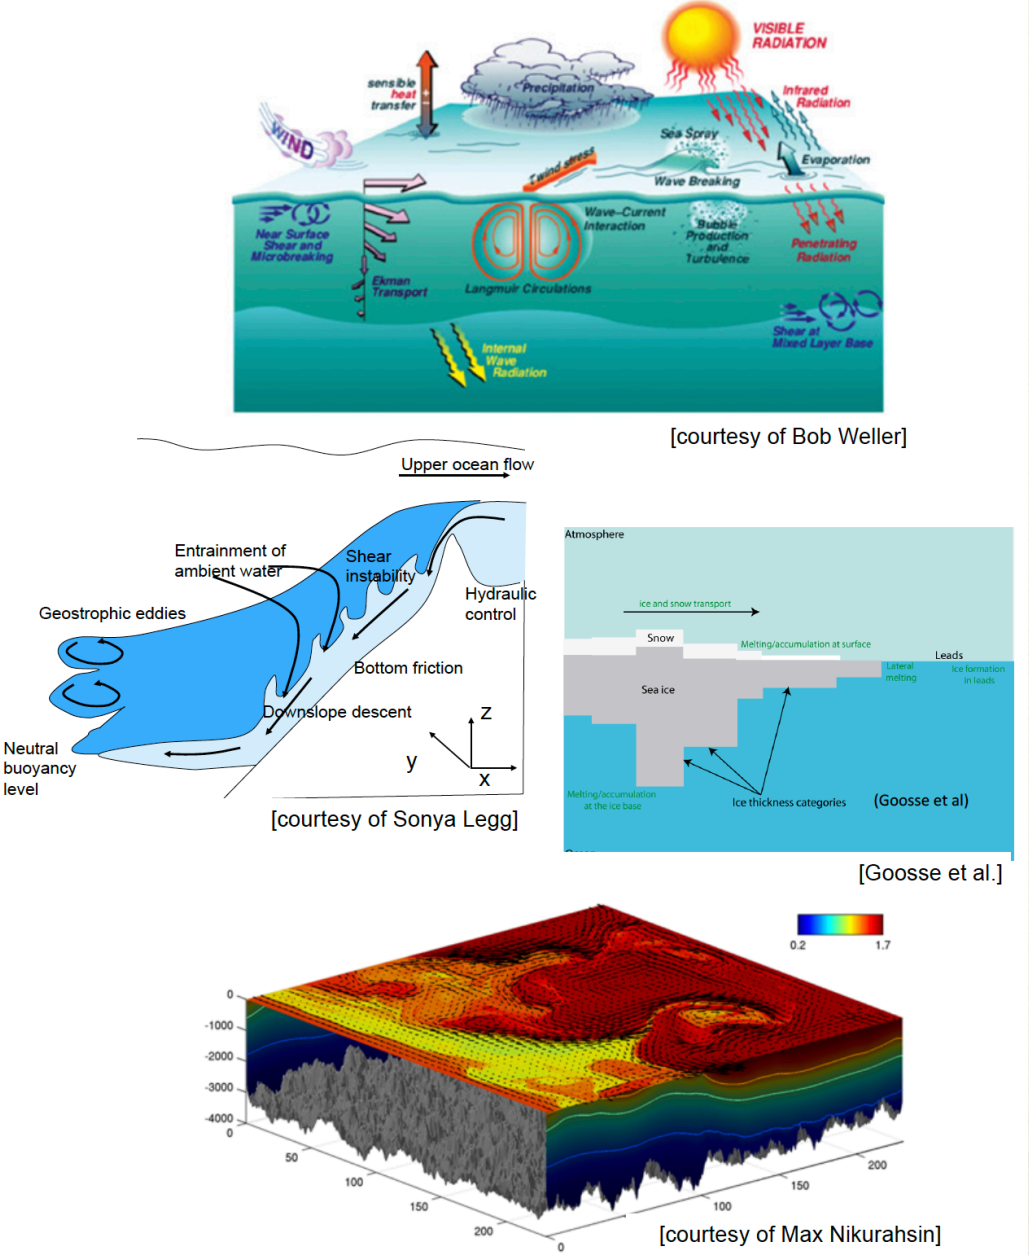
\includegraphics[width=0.4\linewidth]{uploads/Screenshot 2024-11-22 104603.png}\quad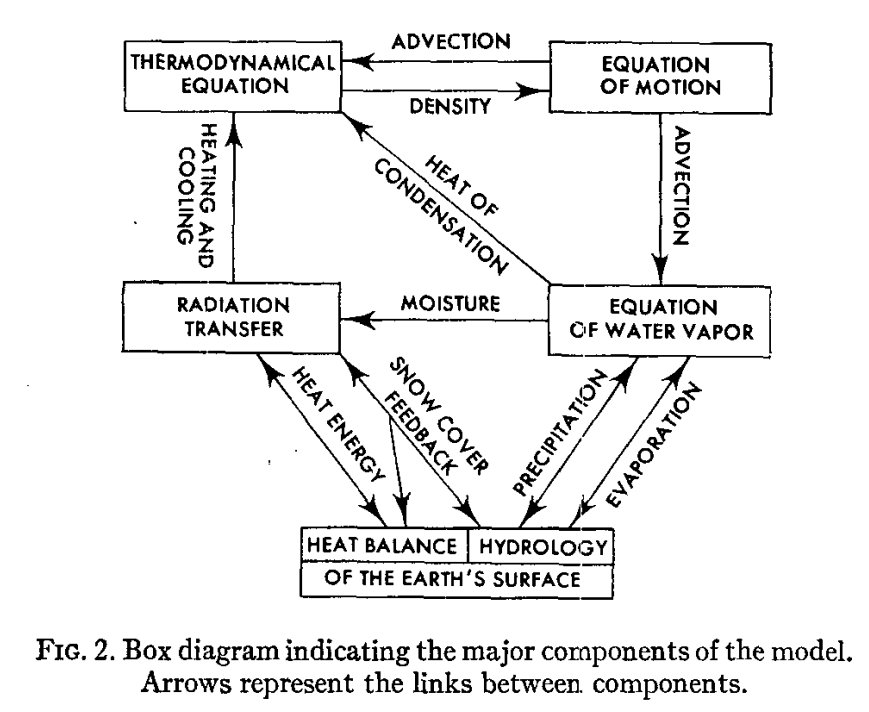
\includegraphics[width=0.35\linewidth]{uploads/Screenshot 2024-11-24 185214.png}
	\caption{Fig.a: Parametrization and eddie problems. Fig.b: Major components of the model}
	\label{...}
\end{figure}


\paragraph{Discretization} \textbf{COMMENT}.



\section{What do we do with climate models?}
\begin{enumerate}
	\item[(i)] Understanding the dynamics of climate
	\item[(ii)] Predict the response of the climate system to perturbations
	\item[(iii)] Challenge limits of predictability
\end{enumerate}
Early attempts where made by integration ad initio, starting from rest, with the objective to simulate the equilibrium climate state (Kasahara and Washington, 1967).
\paragraph{Summary}
Ocean climate models use different grid types to balance computational efficiency and the accurate representation of physical processes. Structured grids, like Cartesian and curvilinear, are efficient and straightforward, making them ideal for large-scale applications but are limited in flexibility and face challenges such as resolution variation near poles. Unstructured grids, composed of irregular shapes like triangles, allow greater adaptability to complex geometries, such as coastlines, but struggle with large-scale geostrophic and advective flows. Emerging adaptive grids dynamically adjust resolution to flow changes but remain in early stages of application. Vertical coordinate systems are crucial for capturing the layered nature of ocean dynamics. Geopotential (depth-based) grids are common in global models for their simplicity but face challenges with mixing. Sigma (terrain-following) systems excel in coastal applications but have accuracy issues with pressure gradients. Isopycnal (density-based) grids are ideal for stratified flows but fail in shallow waters, while hybrid systems combine the strengths of multiple approaches at the cost of computational complexity.

Resolution is critical, as finer grids better resolve mesoscale and sub-mesoscale eddies, essential for modeling ocean dynamics accurately. However, computational constraints limit global models' ability to capture all eddies, necessitating parameterization of unresolved processes such as eddies, surface mixing, and ocean-ice interactions. Parameterization, while indispensable, introduces challenges, especially as models increase resolution and need to represent smaller-scale processes. Advanced techniques are evolving to address these gaps, but significant challenges remain in balancing detail with computational feasibility.


Ocean climate models employ grids to discretize the ocean and simulate its dynamics, but each grid type has limitations that impact their effectiveness. Structured grids, such as Cartesian and curvilinear types, are widely used due to their computational efficiency and straightforward analysis. However, they have inherent challenges, particularly in maintaining uniform resolution. For example, at high latitudes near the poles, grid lines converge, causing distortion in grid cell size and making it harder to achieve uniform resolution across the globe. Unstructured grids, designed with irregular geometries like triangles, offer the flexibility to place high resolution where it is needed most, such as along complex coastlines or over irregular topography. However, these grids face significant challenges in accurately modeling flows dominated by geostrophy (large-scale currents driven by the balance between pressure gradients and Coriolis forces) and advection (transport of properties by the flow). These phenomena dominate large-scale ocean dynamics, and their proper representation is crucial for reliable simulations. The issue arises because irregular grids can struggle to maintain the spatial and numerical consistency required for such processes.

Hybrid coordinate systems combine vertical grid types to optimize performance across different ocean regions. For example, models like HYCOM use geopotential coordinates in the surface mixed layer for simplicity and density-based coordinates below to capture stratified flow dynamics. While this dynamic optimization improves model results by adapting to varying conditions, the process is computationally expensive, requiring frequent updates to grid structures and resolution based on evolving flow conditions. This trade-off between accuracy and computational cost makes hybrid systems challenging to implement widely.

Eddy-resolving models aim to capture mesoscale ocean features, such as large eddies and fronts, which play a critical role in transporting heat and nutrients. However, the statement that "eddy-resolving does not mean all eddies are resolved or that all eddy effects are acting" highlights a subtle limitation: resolving an eddy in a model does not guarantee that its effects (e.g., mixing or momentum transfer) are fully represented. This is because the numerical representation of eddies might still miss critical subgrid-scale processes or interactions with other features. For instance, even at fine resolutions, models might not fully capture the cascading effects of small eddies interacting with larger-scale ocean currents. Thus, while finer resolution improves realism, it cannot eliminate the need for parameterization of unresolved processes.

Parameterization involves representing processes too small or complex to be resolved by the grid, such as the effects of mesoscale eddies, sub-mesoscale turbulence, or ocean-ice interactions. For low-resolution models, the main focus is on capturing mesoscale eddies' effects on energy and tracer distribution, but high-resolution models face additional challenges. For example, they need to parameterize sub-mesoscale processes, such as filaments and internal wave mixing, which become increasingly significant as resolution increases. This introduces resolution-dependent physics, where parameters like viscosity and diffusivity must vary with grid spacing, complicating the modeling process further. Balancing computational efficiency with the need for physical accuracy remains a persistent challenge in this field.

\section{Caos}
It is actually a misnomer, we should really talk about
“sensitivity to initial conditions” (\cite{chaosbook}). The idea had been fluctuated for some time both in
Maxwell and Poincare’ work, probably the first
colourful image is by WS Franklin (1898). Ed Lorenz (1972) after seminal works in 1963 and 1969 introduced in 1972 at 139th Meeting of the AAAS, the concept ‘Does the flap of a buttery’s wings in Brazil set off a tornado in Texas?’.
Deterministic ideas dating to Newton and hyperdeterministic ideas by PS Laplace were put in discussion.
\paragraph{Lorenz System}
\begin{align}\label{eq.lorenz system}
	\frac{dx}{dt}=\sigma(y-x) \\
	\frac{dy}{dt}=x(\rho-z)-y \\
	\frac{dz}{dt}=xy-\beta z
\end{align}
The solutions of this system represent the traveling waves around a cycle of constant latitude.
\begin{align*}
	\dot{x_j}=x_{j-1}(x_{j+1}-x_{j-2})-x_j+F \quad \text{for} \quad j=1,\dots,N \\
	x_{j-N}=x_{j+N}=x_j
\end{align*}
\section{Vorticity dynamics}
\paragraph{What maintains the circulation?} What the factor that maintain the circulation ? starting from the basic structure of the wind, the jet. We need to write the equations of the jet stream. Consider the vorticity budget for a non-divergent case:
\begin{equation}
	\frac{\partial\zeta}{\partial t}=-\vec{v}\cdot\nabla(\zeta+f)
\end{equation}
and introduce now the zonal mean:
\begin{equation}\label{eq.zonal mean}
	\overline{A}=\frac{1}{2\pi}\int_0^{2\pi}Ad\lambda
\end{equation}
separate each field in zonal mean and deviation, $A=\overline{A}+A'$:
$$\frac{\partial}{\partial t}(\overline{\zeta}+\zeta')=-(\overline{u}+u')\frac{\partial}{\partial x}(\overline{\zeta}+\zeta')-(\overline{v}+v')\frac{\partial}{\partial y}(\overline{\zeta}+\zeta'+f_0+\beta y)$$
zonally averaging again:
\begin{equation}\label{eq.average eq}
	\frac{\partial\overline{\zeta}}{\partial t}=-\overline{u}\frac{
		\partial\overline{\zeta}
	}{\partial x}-\overline{v}\frac{\partial\overline{\zeta}}{\partial y}-\beta \overline{v}-\frac{\partial}{\partial y}\overline{v'\zeta'}
\end{equation}
because $\overline{A}=0$, subtracting this equation from the first we get e equation for the perturbation. Note that because in the non-divergent case exist a streamfunction, then $v=\psi_x$ so $\overline{v}=0$ for the periodic boudary conditions:
$$\frac{\partial\zeta'}{\partial t}=-\overline{u}\frac{\partial\zeta'}{\partial x}-v'\frac{\partial\overline{\zeta}}{\partial y}-\beta v'-\frac{\partial}{\partial x}(u'\zeta')-\frac{\partial}{\partial y}(v'\zeta'-\overline{v'\zeta'})$$ for small perturbation we can linearise it:
\begin{equation}
	\frac{\partial\zeta'}{\partial t}=-\overline{u}\frac{\partial\zeta'}{\partial x}-v'\frac{\partial\overline{\zeta}}{\partial y}-\beta v'
\end{equation}
consider the mean equation \ref{eq.average eq}, $\overline{\zeta}=\overline{v}_x-\overline{u}_y$, but the zonal mean of a total derivative in x is zero because of periodic boundary conditions, so $\overline{\zeta}=-\overline{u}_y$:
$$-\frac{\partial}{\partial y}\frac{\partial\overline{u}}{\partial t}=-\overline{u}\frac{\partial\overline{\zeta}}{\partial x}-\overline{v}\frac{\partial\overline{\zeta}}{\partial y}-\beta\overline{v}-\frac{\partial}{\partial y}\overline{v'\zeta'}$$
because it is not divergent, the mean meridional ow can be obtained from a streamfunction, $v=\psi_{x'}\overline{v}$ is also zero, then
$$-\frac{\partial}{\partial y}\frac{\partial\overline{u}}{\partial t}=+\overline{u}\frac{\partial}{\partial x}\frac{\partial\overline{u}}{\partial y}-\frac{\partial}{\partial y}\overline{v'\zeta'}$$
averaging again and remembering that the x-derivative of a zonally averages quantity is zero we get:
\begin{align*}
	\frac{\partial\overline{u}}{\partial t}=\overline{v'\zeta'} \\
	\frac{\partial\overline{u}}{\partial t}=-\frac{\partial}{\partial y}\overline{v'u'}
\end{align*}
This relation shows that the acceleration of the mean ow is caused by the meridional fluxes of momentum. A similar relation can be found for the mean zonal temperature linked to the eddy heat flux. The relation between eddies and jet streams holds also in the three-dimensional case in the Quasi-geostrophic approximation. In this case however we have also non zero
zonal meridional and vertical velocity $(v,w)$.
$$\frac{\partial\overline{u}}{\partial t}=f_0\overline{v}-\frac{\partial}{\partial y}\overline{v'u'}$$
we can then find similar relations for the zonal mean of the temperature:
\begin{equation}\label{eq.zonal mean of temperature}
	\frac{\partial\overline{\theta}}{\partial t}=-N^2\overline{w}-\frac{\partial}{\partial y}\overline{v'\theta'}
\end{equation}
The thermal wind relations link the variables:
\begin{align}\label{eq.thermal wind}
	f_0\frac{\partial\overline{u}}{\partial z}=-\frac{\partial\overline{\theta}}{\partial y} \\
	\frac{\partial\overline{v}}{\partial y}=-\frac{\partial\overline{w}}{\partial z}
\end{align}
\begin{figure}[htp!]
	\centering
	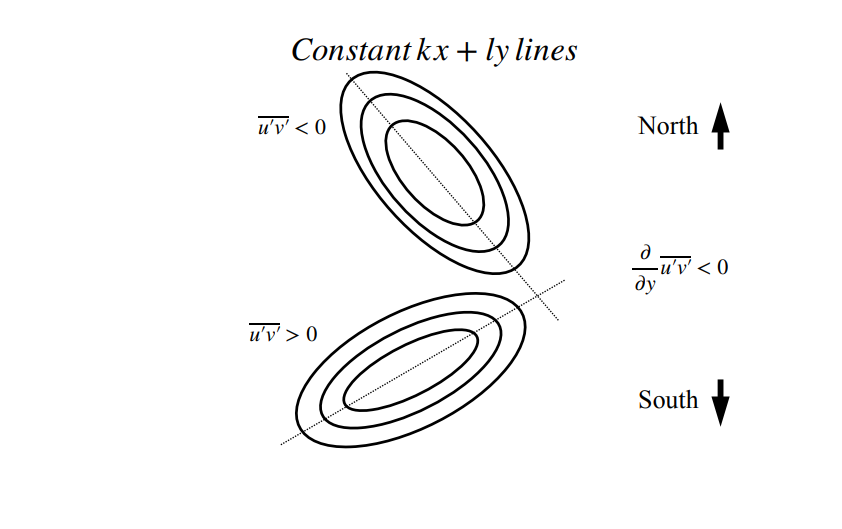
\includegraphics[width=0.5\linewidth]{uploads/Screenshot 2024-11-22 202457.png}
	\caption{Momentum Flux. The meridional transport of momentum depends on the meridional slant of the eddies.}
	\label{fig:enter-label}
\end{figure}

\begin{figure}[htp!]
	\centering
	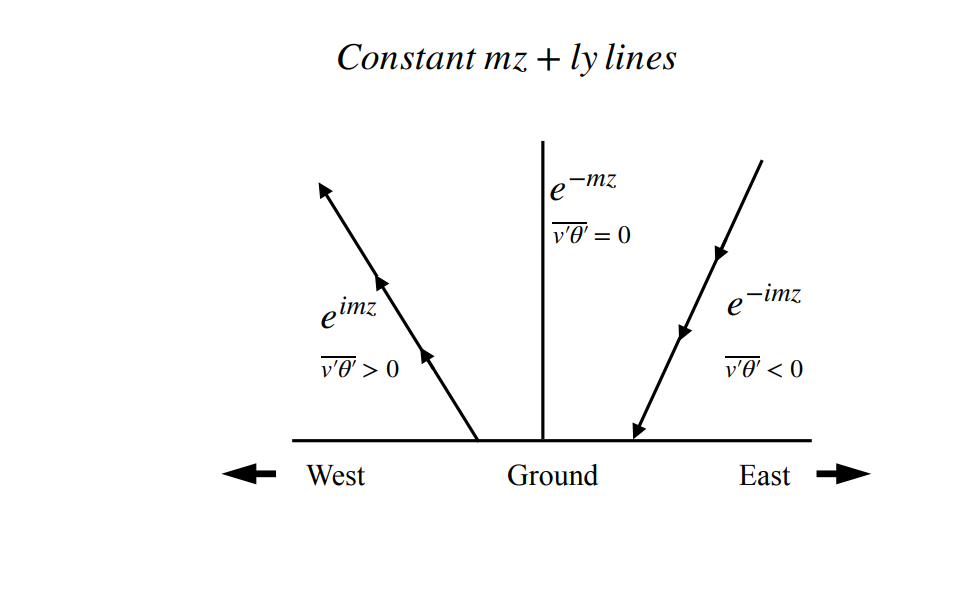
\includegraphics[width=0.5\linewidth]{uploads/Screenshot 2024-11-24 185505.png}
	\caption{Heat flux. The meridional transport of heat depends on the vertical slant of the eddies.}
	\label{fig:enter-label}
\end{figure}
\subsubsection{Kind of eddies}
The models must reproduce the eddy transport properties well otherwise that cannot maintain the basic flow.
\paragraph{Blackmon 1976.}\cite{Black76} Blackmon used spectral methods to decompose the variability of the 500 mb geopotential height field into different spatial and temporal scales. He found:
\begin{itemize}
	\item \textbf{Low-Frequency Variability (Planetary Waves):} Highlighted the dominance of quasi-stationary planetary-scale waves (large-scale undulations in the jet stream).
	\item \textbf{High-Frequency Variability (Synoptic Waves):} Identified transient synoptic-scale systems (e.g., midlatitude cyclones and anticyclones) as major contributors to the atmospheric variability.
\end{itemize}
He demonstrated that most of the variability occurs at intermediate (synoptic) scales. He quantified the distribution of energy across scales, helping to clarify the relative importance of large-scale versus small-scale atmospheric processes. He also found significant geographical differences in the distribution of wave activity, with distinct patterns in storm tracks over the Northern Hemisphere.

\paragraph{Bjerknes.} Jacob Bjerknes, the son of renowned meteorologist Vilhelm Bjerknes, is celebrated for his groundbreaking work in linking El Niño to the Southern Oscillation during the 1960s. While already recognized for his earlier contributions to the theoretical cyclone model developed with the "Bergen School" in the 1920s, Bjerknes turned his attention to understanding the dynamics of the equatorial Pacific.

Bjerknes observed that the sea surface temperatures (SSTs) in the eastern Pacific were unusually cold for such low latitudes, creating a sharp temperature contrast with the warm waters of the western Pacific. This temperature gradient drives a distinct atmospheric circulation, with cool, dry air moving westward along the surface and rising as warm, moist air in the western Pacific. Bjerknes named this systematic east-west atmospheric flow the Walker Circulation.

He proposed that fluctuations in the Walker Circulation could trigger changes in the Southern Oscillation, setting off events associated with El Niño-Southern Oscillation (ENSO). Bjerknes described a feedback loop in which stronger easterly winds enhanced the upwelling of cold water in the east, intensifying the SST gradient and reinforcing the Walker Circulation. Conversely, weaker easterly winds reduced upwelling, diminished the SST gradient, and slowed the circulation. This mechanism explained the alternation between the warm El Niño phase, marked by a weakened Walker Circulation, and the normal cold state of the eastern Pacific associated with the high phase of the Southern Oscillation.

Bjerknes’ insights established the foundation for modern understanding of ENSO, demonstrating how oceanic and atmospheric systems interact in a dynamic feedback loop to shape global climate patterns.
\begin{figure}[htp!]
	\centering
	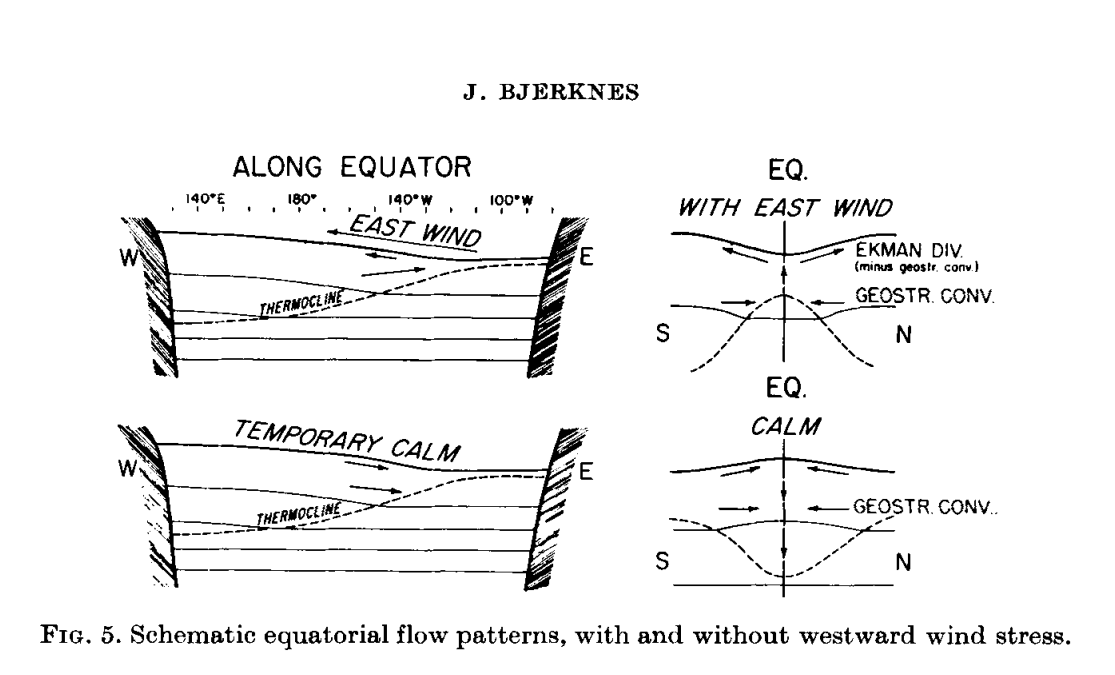
\includegraphics[width=0.5\linewidth]{uploads/Screenshot 2024-11-24 191635.png}
	\caption{The Walker Circulation}
	\label{fig:enter-label}
\end{figure}
The Walker Circulation is driven by the east-west SST gradient along the equatorial Pacific: warm SSTs in the western Pacific generate low-pressure systems, promoting rising air and convection (clouds and rainfall); cool SSTs in the eastern Pacific lead to high-pressure systems, with descending air and dry conditions.
This SST gradient establishes the pressure differences necessary for the Walker Circulation, with surface easterly winds flowing westward and upper-level winds returning eastward: Stronger SST gradients reinforce the Walker Circulation by intensifying convection in the west and upwelling in the east. Weaker SST gradients, such as during El Niño events, disrupt the Walker Circulation by reducing pressure differences, weakening trade winds, and allowing warm water to spread eastward.

Climate forcing (e.g. global warming) modifies SST patterns, disrupting or enhancing the Walker Circulation. Changes in the Walker Circulation, in turn, influence SST distributions and climate change.


\paragraph{Climate forcing.}
Climate forcing refers to external factors that influence the Earth’s climate system, such as greenhouse gas emissions, volcanic eruptions, solar variability, and aerosols. These forces drive changes in sea surface temperatures (SSTs), which play a vital role in regulating global climate by influencing atmospheric circulation, ocean currents, and weather patterns. The interaction between climate forcing and SSTs involves complex mechanisms that include both direct effects and feedback processes.

